\documentclass{article}
\usepackage{soul, xcolor}
\usepackage{float}

\usepackage[sorting = none, style = nature]{biblatex}
\addbibresource{sample.bib}

% Language setting
% Replace `english' with e.g. `spanish' to change the document language
\usepackage[english]{babel}

% Set page size and margins
% Replace `letterpaper' with`a4paper' for UK/EU standard size
\usepackage[a4paper,top=1.5cm,bottom=2cm,left=2cm,right=2cm,marginparwidth=1.75cm]{geometry}


% Useful packages
\usepackage{amsmath}
\usepackage{graphicx}
%\usepackage[colorlinks=true, allcolors=blue]{hyperref}

\title{Comparison between inertial and non-inertial referential frames \\
in human reaching movements}
\author{Mateus Souza Silva}
\date{}
\setlength{\parskip}{0pt}

\begin{document}

\maketitle

\section{Introduction}


Movement is an essential function for the continuity of life, taking in account that we move constantly to perform almost all our activities, so scientists then constantly in search of identifying the optimization principles that are inherent to motor control. To this end, many optimization models have been realized, one of the most discussed in the literature is the \cite{hogan, hoff} start minimization model. This model was developed based on a Cartesian coordinate system and inertial referential, i.e. fixed point of the laboratory as the origin of the system.
\\

However, the referential of the coordinate system used by the motor control is a point under discussion in the biomechanics area, there are authors who consider the inertial referential - \cite{hogan, hoff, miranda, delemos}, however another system widely used in the literature is the joint coordinative system (JCS) that corresponds to a non-inertial referential, in which the movement of a joint is planned based on the previous joint \cite{jcs}.
\\

In order to verify which of these two referential best corresponds to the referential used by motor control during the movement planning process, we will apply the decomposition into movement elements (MED) method \cite{miranda} in order to decompose the movement into a series of elements that will be compared with the theoretical model of movement optimization developed by Flash and Hogan \cite{hogan}.
\\

Our hypothesis is that the inertial reference frame presents results closer to the theoretical optimization model than the non-inertial reference frame (JCS), since in the non-inertial reference frame the motor control would have to perform a much larger information processing, because each joint would have a different non-inertial reference frame system that has its own acceleration.
\\

\section{Methodology}

\subsection{Database}
We will use the human movement database provided by Liang (2020) \cite{database}. In this database, 128 reach movement data files are provided, with the tasks being: touch mouth, back, head, fold towel and grasp and object. The population corresponded to 10 healthy individuals.
\\

The data was collected using the Qualisys movement capture system, originating data in .c3d, full body marker set, and capture frequency of 179 Hz. In this study, as we are not specifically interested in the direction of the reaching movement, we will disregard any difference between the tasks.
\\

For the comparison between the two coordinate systems, we will initially use the HMC2 (Metacarpophalangeal II) markers of the right or left hand depending on which hand will be used to perform the movement. The data already comes from the inertial referential with a fixed origin in the laboratory (because of the camera), to obtain the trajectory with the non-inertial referential, we will use the USP (Ulnar Styloid) marker as the reference.

\subsection{Data treatment}
Initially, to be able to use the data provided in .c3d in R, we need to convert it to .csv. To do this, we developed the function 'c3d\_to\_csv.m' which converts the data from the specific markers we will use into .csv.
\\

Next, to remove instrumental noise, we apply to the data a 10 Hz low-pass filter of 4th order. This filter is a standard already discussed and used in the biomechanics literature \cite{filter}.
\\

Finally, we calculated the velocity time series of each axis through the position time series data and the sampling frequency and then saved the files according to the referential used: inertial - which is the default with origin in the laboratory; and non-inertial - which we used the USP marker as the system origin.

\subsection{Movement element decomposition (MED)}

The movement element decomposition method (MED) consists of decomposing complex movements into simple elements of oscillations, represented by the kinematic curves found between two points of zero velocities in each of the time series of each Cartesian axes. These small oscillations on the Cartesian axes are called movement elements (ME) \cite{miranda}.
\\

Some more complex steps are used to perform this decomposition into movement elements. First, we cannot consider the element to be cut off only when the velocity goes to 0, because in fact, the capture instrument has an experimental error limit (ILE) so that absolute velocities are smaller than the ILE of the velocity can be considered as a zero velocity approximately. Also, movement elements with displacement and duration smaller than a minimum value (1 mm and 100 ms) are considered capture noise and not functional movement elements.
\\

After performing the decomposition into movement elements, we will compare each of these movement elements to the theoretical \cite{hogan, hoff} curve using two metrics, the coefficient of determination \(R^2\) and the similarity index \(W\) described in the literature \cite{delemos}. The higher the coefficient of determination \(R^2\), the greater the correlation between the movement element and the theoretical curve, while the similarity index \(W\) is the opposite, it indicates greater similarity the lower the value.

\section{Results}

By applying MED to all the movement data, we find a total of 12703 movement elements for the inertial referential and 13479 for the non-inertial referential. We then checked the W and R² for each of these elements.
\\

In order to verify which of the two referential had a greater agreement with the profile expected by the theoretical jerk minimization, we applied a mixed linear model, where the fixed factor is given by the referential (inertial or non-inertial) and the random factor is given by the variability of the research subjects. We compared this model with a null model, which only considered the random factor of the individuals, and verified that AIC factor and p-value. 
\\

For W we obtained a p-value = 0, with AIC = 7397.1 for the null model, and 7292.6 for the mixed lm. For the variable R² we also obtained a p-value of 0, with the AIC equal to 12830 for the null model, and 12602 for the mixed lm. As the inertial reference had a lower mean and median and the difference was significant, we conclude that the inertial reference has significantly greater proximity to the theoretical optimization curve.
\\

To present a visualization for this data, in order to soften the effects of individuals, we averaged the values of W and R² for each of the 128 data and then performed the paired difference between the inertial and the non-inertial referential. In figure \ref{fig:boxplot} is represented a boxplot with the paired difference, you can see that the distribution for W is mostly with negative values, indicating that the W of the inertial referential is lower, while for the R² the opposite occurs, the R² of the inertial is mostly higher. Both leading to an agreement that the inertial referential has a better agreement with the theoretical curve.

\begin{figure}[H]
    \centering
    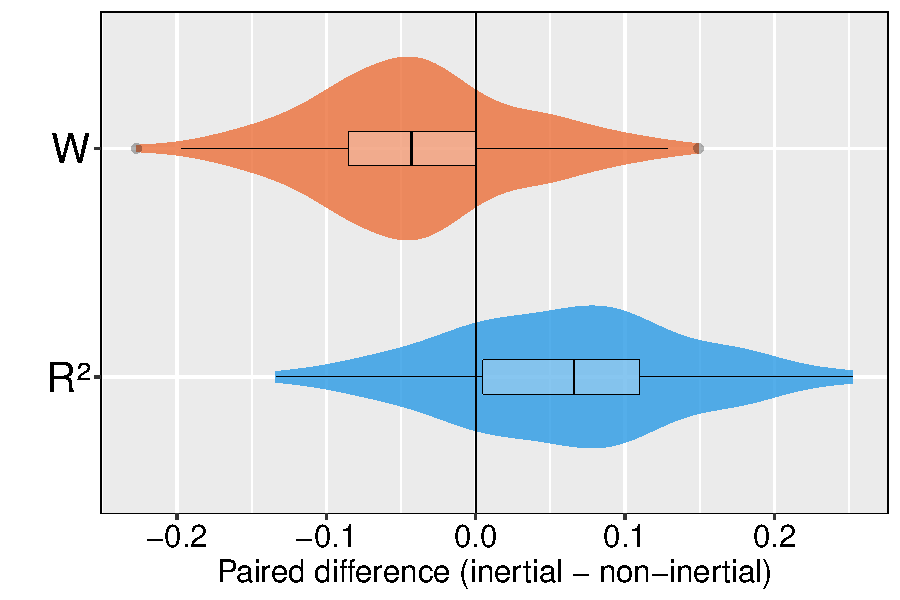
\includegraphics[width=0.8\textwidth]{paired_difference.pdf}
    \caption{Boxplot with violin representation of the paired difference of the indices W and R², where the paired difference means the difference between the mean value of the index in the inertial referential minus the value in the non-inertial.}
    \label{fig:boxplot}
\end{figure}

\section{Discussion and Conclusion}

In this work, it was possible to observe that when comparing the two referential systems, inertial and non-inertial (JCS), using as method the decomposition in elements of movement \cite{miranda} combined with the comparison with the theoretical optimization curve of the start \cite{hogan, hoff}, it is possible to verify that the inertial referential system with fixed origin in the laboratory has a much higher agreement with the theoretical optimization curve, which indicates that this is a referential with greater potential to describe the referential used by the motor control when planning the movements. However, further analysis is necessary to guarantee this result in a more general way;

As a limitation of this study, we have the fact that only simple reaching movements were used, which does not correspond to the whole range of movement possibilities that motor control holds, thus we cannot assume this result as universal, but rather a special case for reaching movements.

As future perspectives, we intend to perform this same comparison method for different referential such as the referential aligned with the vision/head orientation \cite{cabeca}, and with the referential at the center of mass, since for movements in which the individual moves, perhaps considering a fixed point in the room as the origin of the system is not the best approach. Also, modifying the coordinate system is a possibility since taking a spherical coordinate system in the JCS would reduce the number of coordinates from 3 (x, y, z) to 2 (\(\phi\), \(\theta\)) where the radius (R) would be fixed, which could be a potential for the JCS referential.

\printbibliography

\end{document}